%  ~~~~~ INSTRUCTIONS FOR FORMATTING (FOR MORE DETAILS, SEE "Instructions and Cheat Sheet.pdf" in .zip file ~~~~~~
%-----------------------------------------------------------------------------------------------------------------

% COVER PAGE & HEADINGS
% - To begin, please see the "cover.sty" file and enter the details of the following details of the paper:

% -	Add author(s) information:
%     - Underneath the cover page information, you can enter your author and co-author details. 
%     - Please leave these fields blank if you are submitting a new paper with DemRes.  
%--------------------------------------------------------------------------

% REFERENCES 
% - See the “refs.bib” as a guide
%     - Please format using our house style guide (https://www.demographic-research.org/files/DemRes%20Reference%20Guidelines.pdf)
%        - Enter information below, in REFERENCES section.
%--------------------------------------------------------------------------

% APPENDIX (if applicable)
% - Please only add the title "Appendix" or "Appendices" to the TOC (not the subsections). 
%     - All appendices should be alphabetical (e.g., "A. Section name" followed by "Table A-1," etc., then "B. Section name" followed by "Table B-2", etc.).  
%        - Enter information below, in APPENDIX section.

%--------------------------------------------------------------------------

% IN-TEXT 
% - Please leave all packages and encoding as is. 
%     - E.g., the spacing, font size and colour, headings, etc. match our house style and should not be changed. 

%	PRAELEGOMENA  %%
% !TeX encoding = UTF-8
%%	- You must absolutely use unicode encoding (utf8)!

\documentclass[10pt,twoside,reqno]{article}
\raggedbottom

\usepackage[bottom]{footmisc}		%% footnotes
\setlength{\footnotemargin}{0.6em}

\usepackage{blindtext}

\usepackage{DemRes}							%% journal style file

%\usepackage[none]{hyphenat}		%% no hyphenation [!] if style errors occur, solve with \linebreak
\usepackage[utf8]{inputenc}			%% input-encoding: unicode

\makeatletter
\renewcommand*{\@pnumwidth}{3em} %% Width of the box for the page number in the TOC
\setlength{\@fptop}{0pt}				 %%	Floats to the top of the page
%\g@addto@macro\normalsize{%		 %% force equasion spacing to 10pt (font size); it can be helpful to increase the long skips to 12pt to fix spacing issues (of matrices in particular)
%  \setlength\abovedisplayskip{10pt}
%  \setlength\belowdisplayskip{10pt}
%  \setlength\abovedisplayshortskip{10pt}
%  \setlength\belowdisplayshortskip{10pt}
%}
\makeatother

\usepackage{printlen}
\uselengthunit{pt}
\usepackage[hidelinks, pdftitle={\drtitleone}]{hyperref}

%% inhaltsverzeichnis, überschriften
\usepackage{titlesec}
\titleformat{\section}[hang]{\raggedright\normalfont\bfseries\large}{\arabic{section}.}{1ex}{}
\titleformat{\subsection}[hang]{\raggedright\normalfont\bfseries}{\arabic{section}.\arabic{subsection}}{1ex}{}
\titleformat{\subsubsection}[hang]{\raggedright\normalfont\bfseries}{\arabic{section}.\arabic{subsection}.\arabic{subsubsection}}{1ex}{}

\bibpunct [: ] {(} {)} {;} {a} {} {,}

%% insert any additional packages and commands here
% Figures and captions
\usepackage{graphicx}
\graphicspath{{./figures/}}
\usepackage{caption}
\usepackage[font=scriptsize]{subcaption}
\captionsetup[figure]{labelsep=none}
\captionsetup[table]{labelsep=none}

% Math and symbols
\usepackage{amsmath}
\usepackage{bbm}
\usepackage{bm}
\usepackage{calc}

% Tables
\usepackage{array}
\usepackage{booktabs}
\usepackage{makecell}
\usepackage{tabularx}
\usepackage{longtable}
\usepackage{threeparttable}
\usepackage{siunitx}
\sisetup{detect-all}

% Colors
\usepackage[table]{xcolor}
\definecolor{Gray}{gray}{0.9}

% Layout and spacing
\usepackage[margin=1in]{geometry}
\usepackage{setspace}

\usepackage{indentfirst}
\usepackage{afterpage}
\usepackage{adjustbox}
\usepackage{pdflscape}
\usepackage{rotating}

% Floats
\usepackage{float}
\floatstyle{plaintop}
\restylefloat{table}
\usepackage{floatrow}
\usepackage{placeins}

% Text highlighting
\usepackage{soul}

% Bibliography and links
\usepackage[round]{natbib}
\setcitestyle{authoryear}
\usepackage{hyperref}

% Section/title and authors
\usepackage{titlesec}
\usepackage{authblk}

% Importing files
\usepackage{import}

\newcommand\ddfrac[2]{\frac{\displaystyle #1}{\displaystyle #2}}

%%%%%%%%%%%%%%%%%%%%%%

\begin{document}

%%%%%%%%%%%%%%%%%%%%%%%%%%%%%%%%%%%%%%%%%%%%%%%%%%%%%%%%%%%%%%%%%%%%%
%% do not change
\widowpenalty = 10000
\clubpenalty = 10000

\setlength{\parskip}{0ex}
\setlength{\parindent}{.7cm}
\setlength{\bibsep}{.18cm}
\setlength{\belowdisplayskip}{15pt} \setlength{\belowdisplayshortskip}{10pt}
\setlength{\abovedisplayskip}{15pt} \setlength{\abovedisplayshortskip}{10pt}


\title{\textbf{\drtitleone}\vspace{5mm}}
\author{
\ifnum1=\autorzahl
	\autorenitit
\else
	\ifnum2=\autorzahl
		\autoreniitit
	\else
		\ifnum3=\autorzahl
			\autoreniiitit
		\else
			\ifnum4=\autorzahl
				\expandafter\autorenivtit
			\else
				\autorenvtit
			\fi
		\fi
	\fi
\fi
}

\makecover
\newpage
\pagestyle{empty}
\renewcommand{\contentsname}{Contents}
{\footnotesize \tableofcontents}
\newpage
%% until here
%%%%%%%%%%%%%%%%%%%%%%%%%%%%%%%%%%%%%%%%%%%%%%%%%%%%%%%%%%%%%%%%%%%%%

%Placeholders begin with two exclamation marks "!!".

%%%%%%%%%%%%%%%%%%%%%%%%%%%%%%%%%%%%%%%%%%%%%%%%%%%%%%%%%%%%%%%%%%%%%

\setcounter{page}{\drstartpage}							
\maketitle
\thispagestyle{plain}

%%%%%%%%%%%%%%%%%%%%%%%%% ABSTRACT %%%%%%%%%%%%%%%%%%%%%%%%%

\vspace*{-24pt}
\vspace*{5mm}
\setlength{\parskip}{0.5em}
\section*{Abstract}

% - Insert the paper’s information in the ABSTRACT:

\noindent\textbf{BACKGROUND}\\
Household structure impacts the health and well being during pregnancy. Prior research on young women in India documents a shift away from patrilocal extended family residence and toward nuclear households, and suggests trade-offs between autonomy and access to resources in extended vs. nuclear households.
\par
\noindent\textbf{OBJECTIVE}\\
This paper studies whether pregnant women's decision making power and maternal healthcare use differ by household type, and how these relationships have changed over time.
\par
\noindent\textbf{METHODS}\\
Using data from the National Family Health Surveys (NFHS 3, 2005--2006; NFHS 4, 2015--2016; NFHS 5, 2019--2021), we analyze nationally representative samples of pregnant and recently postpartum women. We use linear probability models to compare decision making and maternal healthcare use among pregnant women from nuclear and patrilocal extended households, with and without controls for household wealth. We also assess changes in these relationships over time.
\par
\noindent\textbf{RESULTS}\\
We document a reversal of nuclearization; across the three survey rounds, an increasing proportion of pregnant women in India resides in patrilocal extended households. Across survey rounds, pregnant women in nuclear households have greater decision making power but lower maternal healthcare use than those in patrilocal extended households. Patrilocal extended households have significantly more assets, and differences in asset wealth explain a significant portion of the healthcare advantage. The autonomy gap, however, is not explained by differences in household wealth, and has decreased significantly over time: by 2020 the proportion of pregnant women in patrilocal extended households who reported having no say in their health care, relative to pregnant women in nuclear households, had narrowed to around 6 percentage points, down from 20 percentage points in 2005.
\par
\noindent\textbf{CONCLUSIONS}\\
Lower decision making power does not necessarily translate into lower maternal healthcare use. Autonomy and healthcare use operate through distinct mechanisms, with household resources playing a key role in enabling healthcare use.
\par
% If the contribution splits onto the second page, please add a \pagebreak here.
\noindent\textbf{CONTRIBUTION}\\
This paper provides new evidence on recent changes in household structure among pregnant women in India and suggests that improvements in maternal healthcare use may be driven more by economic resources than by gains in women's autonomy.
 
\vspace*{12pt}

\setlength{\parskip}{0ex}

\pagestyle{fancy}
\setcounter{footnote}{\autorzahl}

%%%%%%%%%%%%%%%%%%%%%%%%%%%% MAIN TEXT %%%%%%%%%%%%%%%%%%%%%%%%%%%

% \newpage % remove if abstract continues to second page
\section{Introduction}\label{Introduction} % remember to change the label if the authors use a different one

Family relationships play a central role in shaping health and well being. Demographers have investigated the relationships between family structure and relationships among household members, on the one hand, and access to resources, social support, and health outcomes, on the other \citep{lindemann2019family, waite2000family, umberson2010social}. For example, marriage has been found to benefit physical health, psychological well being, and even survival in many contexts \citep{ross1990impact, begashaw2016health, lewis2004conceptualization, soulsby2015marriage, robles2014marital}. Further, research finds that marital quality impacts maternal health through the mechanisms of timely and adequate prenatal care, improved emotional well being during and after pregnancy, and reducing high risk behavior like drinking and smoking during pregnancy \citep{alipour2019relationship,rosand2011partner}).

India, home to one in six of the world’s births, provides an important context to examine how household structure impacts maternal health.  Although pregnancy occurs almost exclusively within the context of marriage \citep{banerji2021does}, there is substantial variation in the household structures in which pregnant women reside. Women may live in nuclear households, consisting of only the couple and their children, or they may live in patrilocal extended family households, also called ``joint households.''  Joint households are those in which a woman resides with her husband’s parents, siblings, and other relatives.  Patrilocal extended residence has historically been the normative family structure in India, with land ownership, the responsibility to provide old-age support, and ritual practices organized along male lines \citep{jayachandran2015roots}.  However, a large and modestly increasing fraction of households in India were nuclear -- consisting of a husband, wife, and children -- during the period from 1983 to 2009 \citep{breton2021modernisation}.  A minority of women live in their natal homes, that is, with their own parents, siblings, or relatives.  Their husbands may or may not reside with them.

These family structures shape the social context in which women live, as well as their social status. Newly married women in patrilocal extended households often occupy the lowest position in both gender and generational hierarchies. Because patrilineal societies are organized along the blood lines of men, daughters-in-law in patrilocal extended households are valued for childbearing and labor, but are ultimately replaceable by other women. Ethnographic and sociological work documents that young daughters-in-law are expected to demonstrate deference to senior family members, take on a disproportionate share of domestic labor, and face restrictions on mobility and decision-making \citep{mandelbaum1988women, jeffery1989labour}. These hierarchies are reinforced in India by limited property rights, low female labor force participation, and inheritance systems that privilege senior male members \citep{jayachandran2015roots}. 

The impact on maternal health of a woman's position as daughter-in-law in an extended-family household can occur through many pathways. Other family members may control spending and not invest adequately in maternal health. Daughters-in-law may have limited ability to take rest or travel for healthcare due to their burden of housework. Daughters-in-law may not get enough to eat when they are pregnant. Mothers facing discrimination and stress may develop mental health problems that affect maternal health. \cite{coffey2022mothers} finds that lower women’s status in patrilocal extended households can be linked to lower survival rates and worse health outcomes for children, likely due to worse nutrition among low-status mothers.

In contrast, in nuclear households married women are less likely to face the same pressures from their in-laws. \cite{desai2008negotiated} find that many women in India live separately from their migrant husbands, and that a husband's migration increases a woman's autonomy if they live in a nuclear household. However, for women living in a patrilocal extended households, the shift of power that may occur due to the absence of their husband, is directed primarily towards their in-laws. Similarly, \cite{mookerjee2019gender} finds that exogenous shifts from patrilocal extended to nuclear households increase women’s mobility and participation in decision-making by reducing the control exerted by extended family members.

However, patrilocal households may also offer certain advantages for women, shaping their well-being through multiple mechanisms.  The presence of other adult family members can provide support in the form of shared domestic labor and childcare, which may free up women’s time for other activities \citep{khanna2024role}. Co-residence with extended family members reduces the likelihood of spousal violence \citep{khanna2024role}. Additionally, mothers-in-law and other female household members may be a valuable resource during pregnancy in ensuring that women are getting the care they need \citep{varghese2019coresidence}.  Patrilocal extended households are often characterized by pooled economic resources, inter generational support, and shared domestic labor \citep{wadley1988karimpur}.  

At the same time, hierarchies based on gender and generation may mean that senior family members, particularly mothers-in-law, exercise control over younger women’s mobility and decision making \citep{desai2005women, bloom2001dimensions}. \cite{gupta1999lifeboat} identifies newly married women as the  vulnerable members of the household who are required to demonstrate deference and submission to other family members, and to bear the largest burden of housework. Prior research demonstrates how hierarchies within patrilocal extended households impact women’s health and that of their children. \cite{coffey2022mothers} find that women married to a younger brother have worse maternal health than women married to an older brother in the same household, and that their children have lower chances of survival and poorer growth.

Nuclear households, in contrast, may provide greater scope for spousal communication and individual autonomy, but may lack the economic and caregiving support available in extended families. Married women in nuclear households are less likely to face the same pressure from their in-laws. The absence of a senior kin may increase women’s participation in household decision making \citep{simkhada2010role,char2010influence}. Further, when husbands in nuclear households migrate for work, women become the head of the household, assuming primary responsibility for  household management, further enhancing her decision making authority \citep{desai2008negotiated}. 

This paper investigates how household structure shapes pregnant women's autonomy and their use of maternal health care.  Our findings cohere with characterizations of nuclear and patrilocal extended households in the literature: in all of the three survey rounds that we analyze -- from 2005, 2014, and 2021 -- pregnant women in nuclear households have greater decision-making power relative to pregnant women in patrilocal extended households, but are less likely to use of maternal health care.  We then ask whether and how these relationships have changed in the past two decades.  We find that differences by household type have narrowed, which is consistent with rapid improvement in the accessibility of maternal health care during this period, as well as with important increases in women's decision-making power across household types\citep{ram2026investigation, gandhi2022predictors, muralidharan2017cycling, rai2022use} .

This paper builds upon and dialogs with prior empirical research by \cite{allendorf2013going}, who uses 1992 to 2005 data from India to show that several women's health outcomes were positively associated with patrilocal extended household, rather than nuclear family, residence.  \cite{allendorf2013going}'s paper noted an approximately 8 percentage point increase in the proportion of young women living in nuclear households between 1992 and 2005, and raised the question of how, considering the patrilocal extended household health advantages that she documented, the shift towards nuclear families might impact women's health in the future.  

In contrast, our research, which specifically focuses on pregnant women, finds that in the last two decades, the trend towards nuclear family residence has reversed. Pregnant women are 8 percentage points less likely to be living in nuclear households in 2021 than they were in 2005.\footnote{If, instead of looking at pregnant women, we use \cite{allendorf2013going}'s sample of married women ages 15-29 residing with their husbands, we find the proportion of women living in nuclear households decreased from 36 percent in 2005-06 to 28 percent in 2015-16 and 25 percent in 2019-21.}  However, one thing that remains consistent with the period \cite{allendorf2013going} studied is that patrilocal extended households are wealthier than nuclear families, and wealth is a mediator that explains part of the observed gap in maternal health care use between patrilocal and nuclear households. 

This paper contributes to the literature by documenting a reversal in the trend towards nuclear household structure among pregnant women in India. It shows that pregnant women in patrilocal extended households consistently have lower decision making power than their counterparts in nuclear households, but use maternal healthcare at higher rates. This provides a notable counterexample to the literature which finds or assumes that women's decision making power determines maternal health care use.  In this context, maternal healthcare use is shaped by other factors, such as by economic resources.


\section{Data and Methods}\label{data_and_methods} % remember to change the label if the authors use a different one

\subsection{Data} \label{sec:data}

We use data from India’s National Family Health Surveys (NFHS) rounds 3 (2005–2006), 4 (2015–2016), and 5 (2019–2021). The NFHS is India’s Demographic and Health Survey, a nationally representative cross-sectional survey of households and women aged 15–49. These data are publicly available from \textit{www.dhsprogram.com}.

The sample for our primary analysis on trends in household structure and their relationship with autonomy outcomes are those women who are ever married, currently pregnant\footnote{Appendix Table \ref{tab:earlypregnancy} shows that women who report being one or two months pregnant differ systematically from those reporting three or more months of pregnancy. In particular, early pregnancy is more likely to be recognized or reported among more educated and wealthier women. We therefore exclude women reporting one or two months of pregnancy from the analysis.}, and living in either a nuclear or patrilocal household structure. We exclude women living in natal households (about 15 percent of the sample), as this living arrangement represents a substantively different social context from both patrilocal and nuclear households. For example, \cite{dyson1983kinship} explain that closer ties to the natal families indicate higher autonomy for women.\footnote{The prevalence of visiting to one's natal residence among pregnant women is stable across survey rounds and has further reduced over the survey rounds, as seen in Appendix Figure \ref{fig:bargraph}.  Excluding this group does not affect the interpretation of trends.} For analyses of maternal health care use, instead of focusing on pregnant women, we restrict the sample to ever married women who gave birth in the 3-12 months before the survey.

\subsection{Variables}

\subsubsection{Household structure}
We construct the household structure variable using information on the people residing in the same household as the pregnant woman. We define nuclear households as ones where the woman and her husband are the only two adult members in the household. Patrilocal extended households are defined as the ones where the woman lives with her husband’s adult kin, such as her parent-in-law or adult sibling-in-law. Natal households are those in which the pregnant woman is the daughter or the sister of the household head and none of her husband’s adult kin are present. 

\subsubsection{Sociodemographic variables}  

We define social groups by combining caste and religion, as recommended by the India Human Development Survey (\cite{desai2008india}. Women are classified as Adivasi or Dalit if they report belonging to a Scheduled Tribe or Scheduled Caste, respectively. Muslim women who are not SC/ST are classified as Muslim. Hindu or Sikh women belonging to Other Backward Classes are classified as OBC. Hindu women who are not SC, ST, or OBC are classified as Forward caste. Women who do not fall into these categories (e.g., Christian, Jain, Sikh outside OBC, or no religion) are excluded.\footnote{Only 2.3 percent of pregnant women in NFHS 5 were excluded for this reason.} Uttar Pradesh and Bihar are separated as focus states within regions since they have the highest neonatal mortality in the country (\cite{coffey2025excess}. 

\subsubsection{Outcome variables} \label{sec:outcomes}
To understand women's autonomy during pregnancy, we construct outcomes based on answers to two questions: ``Who usually makes decisions about healthcare for yourself?"  And: ``Who usually makes decisions about visits to your family or relatives?'' We dichotomize these measures by coding women who report that their husband or someone else makes the decision on their behalf as having ‘no say,’ and those who report deciding jointly with their husband or being the only decision maker as ‘some say.’

To measure maternal healthcare use among recently postpartum women, we examine two indicators: birth in a health facility (as opposed to at home) and having 4 or more prenatal visits. The four visit threshold follows the World Health Organization (WHO) and Government of India’s National Health Mission guidelines from 2016.\footnote{In 2016 WHO and NRHM increased the recommended minimum number of visits to 8.  We use 4 because the median pregnant woman in our data was pregnant in 2015.}

\subsubsection{Wealth controls} \label{sec:wealthcontrols}

To capture differences in wealth across household types, we construct a categorical wealth measure based on the full interaction of 8 asset ownership indicators, which has 784 categories. Households are grouped into mutually exclusive categories defined by all combinations of ownership of finished floors, electricity, a radio, a television, a refrigerator, a bicycle, a car, and a latrine or toilet, and these categories are included as fixed effects.

\subsection{Analytical Strategy}
\subsubsection{Patrilocal–nuclear differences and the role of household wealth}

We estimate OLS linear probability models (LPMs) to examine the association between household structure and the four binary outcomes: (1) reporting ``no say'' in decisions about the respondent's own healthcare, (2) reporting ``no say'' in decisions about visits to family or relatives, (3) having an institutional delivery (birth in a health facility), and (4) receiving at least four prenatal visits. We use LPMs because the coefficients can be directly interpreted as percentage point differences, which facilitates comparison across outcomes and survey rounds. In our data, the outcomes are not extremely rare, so linear models provide a reasonable approximation.

For woman $i$ in state $s$, our baseline specification is:

\begin{equation} \label{eq:nocontrols}
Y_{is} = \beta_0 + \beta_1 \text{Patrilocal}_{is} + \mu_s + \epsilon_{is},
\end{equation}

where $i$ indexes women and $s$ indexes states. $Y_{is}$ denotes the outcomes described above, $\text{Patrilocal}_{is}$ is an indicator for residing in a patrilocal extended household (with nuclear households as the reference category), $\mu_s$ are state fixed effects, and $\epsilon_{is}$ is an error term. We estimate this equation separately for each NFHS round: NFHS-3 (2005--06), NFHS-4 (2015--16), and NFHS-5 (2019--21) to examine how the relationships between household structure and the outcomes change over time.

To assess the role of household economic status, we estimate an additional specification that includes $\lambda_{g(i)}$, the wealth group fixed effects described above:

\begin{equation} \label{eq:controls}
Y_{is} = \beta_0 + \beta_1 \text{Patrilocal}_{is} + \lambda_{g(i)} + \mu_s + \epsilon_{is}.
\end{equation}

In all models, we report standard errors clustered at the primary sampling unit level to account for within-cluster correlation of outcomes.\footnote{All models account for the NFHS complex survey design using sampling weights and stratification.}

\subsubsection{Changes in patrilocal–nuclear differences over time}

To examine how differences between patrilocal extended and nuclear households evolve over time, we estimate models that allow the association between household structure and outcomes to vary across survey rounds. Specifically, for comparisons between 2005-2006 and 2015-2016, as well as 2015-2016 and 2019-2021, we estimate:

\begin{equation} \label{eq:tworounds}
Y_{is} = \alpha + \beta \,\text{Patrilocal}_i + \gamma \,\text{LaterRound}_t
+ \delta \,(\text{Patrilocal}_i \times \text{LaterRound}_t)
+ \lambda_{g(i)} + \mu_s + \varepsilon_{is},
\end{equation}


where $\text{LaterRound}_t$ is an indicator for the later survey round in the comparison. The coefficient of interest $\delta$ captures the change in the patrilocal-nuclear gap between the two survey rounds. As in the main specification, $\lambda_{g(i)}$ denotes wealth-group fixed effects, and $\mu_s$ denotes state fixed effects. This approach allows us to directly test whether the patrilocal–nuclear gap changes across survey rounds, and to assess the statistical significance of these changes.

We also estimate a pooled specification including all three survey rounds to assess changes in the patrilocal-nuclear gap across rounds while using the full sample. The equation is:

\begin{equation} \label{eq:stacked}
\begin{aligned}
Y_{is} = \alpha 
&+ \beta \,\text{Patrilocal}_i
+ \gamma_4 \,\text{NFHS4}_t
+ \gamma_5 \,\text{NFHS5}_t \\
&+ \delta_4 \,(\text{Patrilocal}_i \times \text{NFHS4}_t)
+ \delta_5 \,(\text{Patrilocal}_i \times \text{NFHS5}_t) \\
&+ \lambda_{g(i)} + \mu_s + \varepsilon_{is}.
\end{aligned}
\end{equation}

2005-2006 is the omitted category; NFHS4 refers to 2015-2016, and NFHS5 refers to 2019-2021. $\lambda_{g(i)}$ denotes wealth-group fixed effects, and $\mu_s$ denotes state fixed effects. The reported coefficients $\delta_4$ and $\delta_5$ measure changes in the patrilocal-nuclear gap relative to the gap in 2005-2006.

\section{Results}
\subsection{Trends in Patrilocal Residence}

Table \ref{tab:patrilocal_subgroups} shows that the share of pregnant women living in patrilocal extended households increased from 61 percent in 2005–2006 to 71 percent in 2019–2021. This increase is observed across all major social groups except Adivasi women, with particularly large increases among OBC women (15 percentage points), and smaller increase for Muslim women at 3 percentage points.

Patrilocal residence increased in all regions except the East. In 2019-2021, patrilocal residence is highest in the North and West (79 and 82 percent, respectively), but even areas with comparatively lower baseline levels of patrilocal residence such as Northeast and South showed a noticeable increase in patrilocal residence.  

Patrilocal residence varies sharply by age and parity. Younger women are substantially more likely to live in patrilocal extended households than older women: in 2019–2021, 83 percent of pregnant women aged 15–19 reside in patrilocal households, compared to less than 40 percent among women aged 40–44. Similarly, women with lower parity are more likely to reside in patrilocal households. These patterns are consistent with the view that patrilocal extended household residence is most common in the early stages of marriage and childbearing. While it declines with age and parity, increases over time are observed across most age and parity groups. 

\begin{table}[H]
\sansmath
\sffamily
\captionsetup{style=CAPFIG}
\caption{Proportion of pregnant women in patrilocal extended households is increasing among all subgroups}
\label{tab:patrilocal_subgroups}
\vspace{-4pt}

\begin{scriptsize}
\setlength{\tabcolsep}{6pt}
\renewcommand{\arraystretch}{1.3}
\centering
\input{tables/DR/table 1 patrilocal in subgroups}
\end{scriptsize}


\vspace{1ex}
\small\scriptsize{\textsf{\textit{Note}: Data is from NFHS rounds 3, 4, and 5.}} 
\small\scriptsize{\textsf{The sample is restricted to women in either nuclear or patrilocal extended household structures, and women who report being three or more months pregnant when surveyed.}}
\newline\small\scriptsize{Stars indicate the statistical significance of the difference between the 2005--2006 and 2019--2021 estimates. P-values are from weighted linear probability models regressing patrilocal extended household residence on an indicator for 2019--2021, restricted to the relevant subgroup. Standard errors are clustered at the primary sampling unit level. \textsf{*$p<0.1$, **$p<0.05$, ***$p<0.001$}}
\newline\small\scriptsize{\textsf{$^1$ Focus states refer to Uttar Pradesh and Bihar, two Indian states that have a large burden of poor maternal health outcomes.}}

\end{table}

\subsection{Sample means by household structure}

Table \ref{tab:sumstats} presents summary statistics for autonomy, maternal healthcare use, and wealth outcomes by household structure. Among currently pregnant women, there are large and persistent differences in decision-making power by household type. In 2005–2006, 52 percent of women in patrilocal extended households report having no say in their own healthcare, compared to 32 percent of women in nuclear households. By 2019–2021, these shares decline to 25 percent. While autonomy improves substantially over time for both groups, the gap between household types narrows considerably, from 20 percentage points in 2005–2006 to 7 percentage points in 2019–2021. A similar pattern is observed for women’s ability to visit family and friends, where differences of comparable magnitude persist across all survey rounds.

In contrast, maternal healthcare use is higher for women in patrilocal extended households. Among women who gave birth in the 3–12 months preceding the survey, 45 percent of women in patrilocal households delivered in a health facility in 2005–2006, compared to 34 percent in nuclear households. By 2019–2021, although institutional delivery rates increased dramatically for both groups, to 93 percent in patrilocal households and 86 percent in nuclear households, the advantage for patrilocal households remained. A similar pattern is observed for prenatal care: the share of women receiving four or more visits rises from 40 to 61 percent in patrilocal households and from 31 to 53 percent in nuclear households over the same period. Thus, while overall access to maternal healthcare improved substantially, differences by household structure persist.

Patterns in maternal healthcare use mirror differences in household wealth between household structures. Across all survey rounds and for nearly all indicators, women in patrilocal extended households are more likely to live in households with higher asset ownership and better housing conditions. For example, in 2019–2021, 61 percent of pregnant women in patrilocal households live in homes with finished floors compared to 48 percent in nuclear households, and 81 percent in patrilocal extended household have access to a toilet or latrine compared to 68 percent in nuclear households. Ownership of consumer durables such as televisions and refrigerators is also substantially higher in patrilocal households.


\begin{table}[H]
\sansmath
\sffamily
\captionsetup{style=CAPTAB}
\caption{Pregnant women in patrilocal extended households are advantaged in wealth and maternal healthcare use, but disadvantaged in autonomy outcomes}
\label{tab:sumstats}
\vspace{-4pt}

\begin{scriptsize}
\setlength{\tabcolsep}{3.5pt}
\renewcommand{\arraystretch}{1.15}

\input{tables/DR/table 1 summary stats by hhstruc}

\end{scriptsize}

\vspace{1ex}
\small\scriptsize{\textsf{\textit{Note}: Data are from NFHS rounds 3, 4, and 5.}} \small\scriptsize{\textsf{Stars indicate the statistical significance of the difference between nuclear and patrilocal extended households. P-values are from weighted linear probability models regressing each outcome on an indicator for patrilocal extended household residence.}} \small\scriptsize{\textsf{*$p<0.1$, **$p<0.05$, ***$p<0.001$.}}
\newline\small\scriptsize{\textsf{The sample is restricted to ever-married women in either nuclear or patrilocal extended household structures. The pregnant sample includes women who report being three or more months pregnant at the time of the survey and who were asked the questions ``Who usually makes decisions about healthcare for yourself?'' and ``Who usually makes decisions about visits to your family or relatives?''}} \small\scriptsize{\textsf{The outcomes ``No say in own healthcare'' and ``No say in visits to family/friends'' are constructed from these questions. The recent birth sample includes ever-married women who gave birth 3--12 months before the survey.}}

\end{table}


% \begin{table}[H]
% \sansmath
% \sffamily
% \captionsetup{style=CAPTAB}
% \caption{Pregnant women in patrilocal extended households are advantaged in wealth and maternal healthcare use, but disadvantaged in autonomy outcomes}
% \label{tab:sumstats}
% \vspace{-4pt}

% \begin{center}
% \begin{scriptsize}
% \setlength{\tabcolsep}{3pt}
% \renewcommand{\arraystretch}{1.15}

% \begin{tabular}{>{\raggedright\arraybackslash}p{2.8cm}ccccccccc}
% \toprule
%  & \multicolumn{3}{c}{NFHS-3 (2005--2006)} & \multicolumn{3}{c}{NFHS-4 (2015--2016)} & \multicolumn{3}{c}{NFHS-5 (2019--2021)} \\
% \cmidrule(lr){2-4} \cmidrule(lr){5-7} \cmidrule(lr){8-10}
%  & Nuclear & \shortstack{Patrilocal\\Extended} & Sig. & Nuclear & \shortstack{Patrilocal\\Extended} & Sig. & Nuclear & \shortstack{Patrilocal\\Extended} & Sig. \\
% \midrule
% \textbf{\shortstack[l]{Autonomy measures\\(pregnant sample)}}&&&&&&&&&\\
% No say in own healthcare&0.32&0.52&***&0.26&0.32&***&0.18&0.25&***\\
% No say in visits to family/friends&0.32&0.56&***&0.25&0.35&***&0.17&0.25&***\\
% &&&&&&&&&\\
% \textbf{\shortstack[l]{Healthcare measures\\(recent birth sample)}}&&&&&&&&&\\
% Birth in a health facility&0.34&0.45&***&0.77&0.86&***&0.86&0.93&***\\
% 4+ prenatal visits&0.31&0.40&***&0.45&0.55&***&0.53&0.61&***\\
% &&&&&&&&&\\
% \textbf{\shortstack[l]{Wealth measures\\(pregnant sample)}}&&&&&&&&&\\
% Finished floor&0.32&0.43&***&0.46&0.54&***&0.51&0.59&***\\
% Electricity&0.60&0.70&***&0.80&0.88&***&0.94&0.97&***\\
% Owns radio&0.26&0.38&***&0.06&0.12&***&0.05&0.08&**\\
% Owns TV&0.31&0.51&***&0.48&0.67&***&0.54&0.68&***\\
% Owns refrigerator&0.07&0.18&***&0.18&0.36&***&0.28&0.44&***\\
% Owns bicycle&0.35&0.58&***&0.38&0.55&***&0.37&0.50&***\\
% Owns car&0.01&0.04&***&0.03&0.08&***&0.07&0.12&***\\
% Uses toilet/latrine&0.43&0.49&***&0.56&0.61&***&0.78&0.83&***\\
% Owns land&.&.&&0.33&0.29&**&0.40&0.33&***\\
% &&&&&&&&&\\
% \textbf{\shortstack[l]{Wealth measures\\(recent birth sample)}}&&&&&&&&&\\
% Finished floor&0.32&0.42&***&0.44&0.54&***&0.48&0.61&***\\
% Electricity&0.53&0.65&***&0.78&0.88&***&0.93&0.97&***\\
% Owns radio&0.22&0.36&***&0.05&0.09&***&0.03&0.04&***\\
% Owns TV&0.28&0.48&***&0.47&0.68&***&0.49&0.71&***\\
% Owns refrigerator&0.07&0.16&***&0.15&0.31&***&0.23&0.42&***\\
% Owns bicycle&0.44&0.63&***&0.45&0.57&***&0.44&0.56&***\\
% Owns car&0.01&0.03&***&0.02&0.07&***&0.04&0.08&***\\
% Uses toilet/latrine&0.34&0.39&***&0.47&0.57&***&0.68&0.81&***\\
% Owns land&.&.&&0.32&0.31&&0.36&0.33&**\\
% &&&&&&&&&\\
% \textbf{\shortstack[l]{N\\(pregnant sample)}}&1,752&2,572&&1,249&2,585&&961&2,008&\\
% &&&&&&&&&\\
% \textbf{\shortstack[l]{N\\(recent birth sample)}}&2,950&4,013&&12,762&22,871&&10,776&21,257&\\
% &&&&&&&&&\\
% \bottomrule
% \end{tabular}

% \end{scriptsize}
% \end{center}

% \vspace{1ex}
% \small\scriptsize{\textsf{\textit{Note}: Data is from NFHS rounds 3, 4, and 5. *$p<0.1$, **$p<0.05$, ***$p<0.001$}}
% \newline\small\scriptsize{\textsf{The pregnant sample includes ever-married women who report being three or more months pregnant at the time of the survey and who were asked the questions ``Who usually makes decisions about healthcare for yourself?" and ``Who usually makes decisions about visits to your family or relatives?'' from which we construct the outcomes "No say in own healthcare" and "No say in visits to family/friends".}}
% \newline\small\scriptsize{\textsf{The recent birth sample includes ever-married women who gave birth 3--12 months before the survey.}}

% \end{table}




\subsection{Patrilocal–nuclear differences and the role of household wealth}

Figure \ref{fig:regresults} presents estimates of the patrilocal coefficient (relative to nuclear households) from equations \ref{eq:nocontrols} and \ref{eq:controls} for each outcome and survey round, with and without wealth controls. These coefficients represent percentage point differences in outcome probabilities between women in patrilocal and nuclear households.

\subsubsection{ Maternal healthcare use outcomes}

In models without wealth controls, women in patrilocal extended households exhibit higher levels of maternal healthcare use across survey rounds. In 2005–2006, women in patrilocal households are 11 percentage points more likely to deliver in a health facility than those in nuclear households. This advantage declines over time, to 7.4 percentage points in 2015–2016 and 5.2 percentage points in 2019–2021. A similar pattern is observed for prenatal care: in 2005–2006, patrilocal residence is associated with a 8.8 percentage point higher likelihood of receiving four or more prenatal visits, declining to 5.4 percentage points by 2019–2021.

Controlling for wealth substantially attenuates these differences, indicating that a large share of the advantage in maternal healthcare use among patrilocal households is explained by differences in household economic resources. For institutional delivery, the coefficient declines from 11 to 4.2 percentage points in 2005–2006, from 7.6 to 3.6 percentage points in 2015–2016, and from 5.2 to 2.9 percentage points in 2019–2021. In other words, accounting for wealth explains a substantial share—roughly half—of the gap in institutional delivery between patrilocal and nuclear households across survey rounds. For prenatal care, the corresponding reductions are from 8.8 to 2.4 percentage points in 2005–2006, from 7.9 to 3.9 percentage points in 2015–2016 and from 5.4 to 3.2 percentage points in 2019–2021.

\subsubsection{Autonomy outcomes}

In contrast, patrilocal residence is consistently and robustly associated with lower levels of decision-making power. In 2005–2006, women in patrilocal extended households are 17 percentage points more likely to report having no say in their own healthcare and 21.5 percentage points more likely to report no say in visits to family and friends. These gaps decline substantially over time but remain non-trivial: by 2019–2021, the corresponding differences are 5.5 percentage points for no say in own healthcare, and 6.7 percentage points for no say in visits to family and friends. 

Controlling for wealth does not attenuate these differences. For both autonomy outcomes, the estimated coefficients remain similar in magnitude with and without wealth controls. This pattern indicates that, unlike maternal healthcare use differences in decision-making power between patrilocal and nuclear households are not explained by differences in household economic resources.

\begin{figure}[H]
\begin{flushleft}
\captionsetup{style=CAPFIG}
\caption{Estimated differences in autonomy and healthcare use outcomes for women living in patrilocal extended households relative to nuclear households}
\label{fig:regresults}
\vspace{-4pt}

\begin{center}
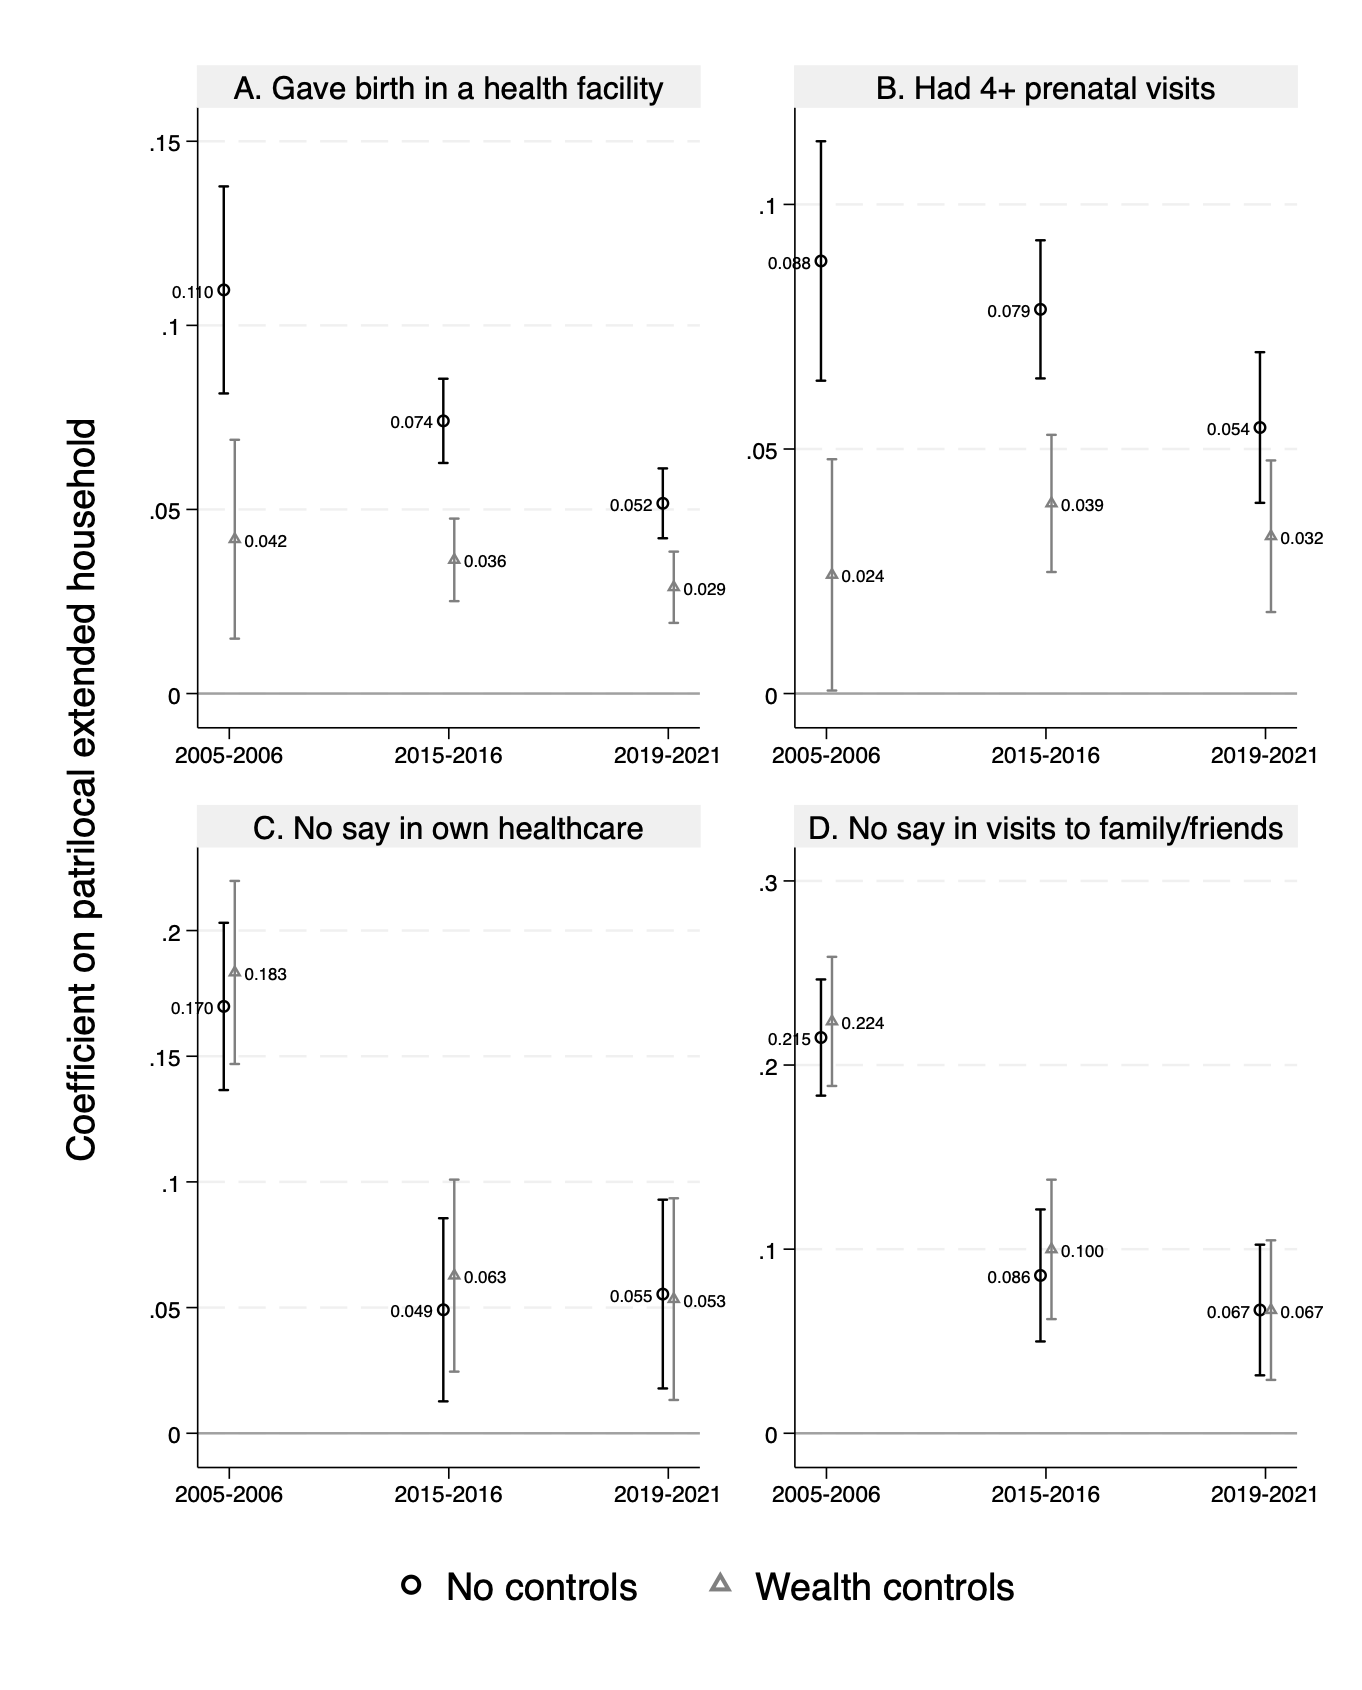
\includegraphics[width=\textwidth]{figures/DR/figure 1 regression coefficients with and without controls.png}
\end{center}

\vspace{1ex}
\small\scriptsize{\textsf{\textit{Note}: Data are from NFHS rounds 3, 4, and 5.}}
\newline\small\scriptsize{\textsf{Points represent the coefficient $\beta$ on the patrilocal extended household indicator from the linear probability models shown in equations \ref{eq:nocontrols} and \ref{eq:controls}. Intervals represent 95\% confidence intervals on $\beta$.}}
\newline\small\scriptsize{\textsf{All four panels restrict the sample to ever-married women living in either nuclear or patrilocal extended household structures. Panels A and B use the recent birth sample, defined as ever-married women who gave birth 3--12 months before the survey.}}
\newline\small\scriptsize{\textsf{Panels C and D use the pregnant sample, defined as women who report being three or more months pregnant at the time of the survey and who were asked the decision-making questions ``Who usually makes decisions about healthcare for yourself?'' and ``Who usually makes decisions about visits to your family or relatives?''}}
\newline\small\scriptsize{\textsf{The outcomes ``No say in own healthcare'' and ``No say in visits to family/friends'' are constructed from these decision-making questions. Sample sizes for each regression match the number of women in the relevant subsample described in Table \ref{tab:sumstats}.}}

\end{flushleft}
\end{figure}


\subsection{Changes in patrilocal–nuclear differences over time}

Table \ref{tab:narrowinggaps} presents estimates of changes in the gap between patrilocal extended and nuclear households over time. Consistent with the descriptive results, differences in women’s autonomy narrow substantially across survey rounds. Between 2005–2006 and 2015–2016, the gap in having no say in healthcare decisions declines by 10.6 percentage points, while the gap in having no say in visiting family and friends declines by 11.7 percentage points. Little additional change occurs between 2015–2016 and 2019–2021 for these autonomy outcomes, but over the full period, the autonomy gaps decline by 13.5 and 17.3 percentage points, respectively.

In contrast, changes in gaps between women in patrilocal extended and nuclear households for maternal healthcare use outcomes are smaller. For institutional delivery, the gap declines by 2.3 percentage points between 2015–2016 and 2019–2021 and by 3.6 percentage points over the full period. For prenatal care, the gap declines by 2.6 percentage points in the later period, but this change is not large enough to generate a statistically significant decline over the full sample period. Overall, convergence in maternal healthcare use across household structures is more limited than for autonomy. 

Appendix table \ref{tab:decomposition} shows that changes in household structure  composition explains little of the improvement in autonomy and maternal health outcomes with most gains driven by within household type changes. Further in appendix table \ref{tab:proppatrilocal} we observe that declining fertility reflected in first parity pregnancies accounts for a significant portion of the increase in patrilocal residence. Together these results suggests that while improvements in outcomes are not driven by shifts in household composition changes in fertility behavior plays an important role in shaping residence pattern.

\begin{table}[H]
\sansmath
\sffamily
\captionsetup{style=CAPTAB}
\caption{The gap between patrilocal extended and nuclear households in women's autonomy and health care use in narrowing across survey rounds}
\label{tab:narrowinggaps}
\vspace{-4pt}

\begin{scriptsize}
\setlength{\tabcolsep}{6pt}
\renewcommand{\arraystretch}{1.6}
\centering
\begin{tabular}{lcccc}
\toprule
 & \multicolumn{1}{c}{\shortstack{$\delta$ (Eq.~\ref{eq:tworounds})\\2005--2006 vs.\\2015--2016}} & \multicolumn{1}{c}{\shortstack{$\delta$ (Eq.~\ref{eq:tworounds})\\2015--2016 vs.\\2019--2021}} & \multicolumn{1}{c}{\shortstack{$\delta_4$ (Eq.~\ref{eq:stacked})\\2005--2006 vs.\\2015--2016}} & \multicolumn{1}{c}{\shortstack{$\delta_5$ (Eq.~\ref{eq:stacked})\\2005--2006 vs.\\2019--2021}} \\\\
\midrule
No say in visits to family/friends$^1$&-0.127***&-0.012&-0.127***&-0.177***\\
Gave birth in a health facility$^2$&-0.059*&0.030&-0.054*&-0.043\\
No say in own healthcare$^1$&-0.074***&0.004&-0.077***&-0.107***\\
Had 4+ prenatal visits$^2$&0.001&0.046&-0.006&0.020\\
&(0.031)&(0.034)&(0.031)&(0.033)\\
&(0.021)&(0.022)&(0.021)&(0.020)\\
&(0.033)&(0.041)&(0.032)&(0.037)\\
&(0.021)&(0.021)&(0.020)&(0.020)\\
&N = 12,994&N = 10,832&N = 17,761&N = 17,761\\
&N = 4,708&N = 3,605&N = 6,185&N = 6,185\\
&N = 4,709&N = 3,606&N = 6,186&N = 6,186\\
&N = 12,994&N = 10,832&N = 17,761&N = 17,761\\
\bottomrule
\end{tabular}

\end{scriptsize}

\vspace{1ex}
\small\scriptsize{\textsf{\textit{Note}: Data is from NFHS rounds 3, 4, and 5.}}
\newline\small\scriptsize{\textsf{*$p<0.1$, **$p<0.05$, ***$p<0.001$}}
\newline\small\scriptsize{\textsf{$^1$ Uses the sample of ever-married women who report being 3 or more months pregnant at the time of the survey.}}
\newline\small\scriptsize{\textsf{$^2$ Uses the sample of ever-married women who report having given birth 3 to 12 months before the survey.}}

\end{table}

\section{Discussion}

We use the most recent three waves of NFHS data to document a reversal in the trend towards nuclear family residence that \cite{allendorf2013going} documented for the period 1991 to 2005.  This trend is driven by an increase in the proportion of pregnant women living in patrilocal extended households, rather than an increase in the proportion of women living in natal households. Our results are surprising in the context of an influential prior literature that associates modernization with a shift towards nuclear households.  They are consistent with \cite{pesando2018global} who find that in more recent data, there is no association between a country's level of human development and the share of women living in nuclear households.

The prior literature on family in India finds that extended families are less egalitarian than nuclear families; indeed, newly married women in patrilocal households occupy subordinate positions relative to their in-laws and their husbands older brothers and their wives. Senior family members often dictate the details of the daily lives of co-resident daughters-in-law. Our findings are consistent with these long-standing gender and age hierarchies: pregnant women in extended families have less say in their own healthcare and visits to family and friends than pregnant women in nuclear households, even controlling for wealth differences across these households. Yet, pregnant women in extended families are more likely to use prenatal care and give birth in a health facility.  Differences in household level wealth do explain much of this gap. 

Our results should be interpreted in the context of broad improvements in the availability of healthcare and of changes in the underlying determinants of women's status.  The time window we study begins in 2005, when the central government launched the National Rural Health Mission to expand contraceptive, prenatal, birth, and postnatal services.  As an illustration of these programs' reach, between 2005 and 2021, the proportion of women who gave birth in health facilities increased from about 40\% to about 90\% \citep{IIPS2007NFHS3,IIPS2021NFHS5}.  \cite{char2010influence} post that these programs not only shaped access to reproductive healthcare, but also reduced the influence of mothers-in-law over the child-bearing patterns of their sons and daughters-in-law.  Over the same period, the median pregnant woman's years of schooling increased from 3 years to 9 years, and the average gap between her education and her husband's decreased from 2.1 year in 2005-06 to 0.6 years in 2019-2021.  This is not to say that education necessarily increases a woman's autonomy within the home: \cite{srivastava2020time} compares women who are more or less educated than their co-resident mothers-in-law and finds that more educated women do not do less housework.  Households also got richer during this period in ways that shaped women's work: in 2005, 17.09\% of extended households in which a pregnant woman resided primarily used lpg gas  for cooking, compared to 48\% in 2021.  The consequences of increasing patrilocal extended family residence would almost certainly have been different in the absence of these important society-level changes.

This study has a few limitations. Our measures capture use, but not the quality, of maternal healthcare. Four or more prenatal visits do not guarantee adequate, continuous, or comprehensive care. Similarly, the quality of institutional delivery varies across facilities.  In some settings, home birth is associated with lower neonatal mortality than private hospital birth \citep{coffey2025excess}. Further, our measures of autonomy rely on self-reported decision-making authority. They may not capture informal influence or everyday negotiations within the household. NFHS data are cross-sectional and capture household structure only at the time of the survey. However, residence arrangements around marriage and childbirth can be fluid. Women may move between households frequently during this period. This movement could lead to error in our measurement household structure.  The fact that natal family residence among pregnant women changes little across the three survey waves gives us more confidence in our results.

Although it is beyond the scope of this paper to investigate the reasons for pregnant women's increasing residence in patrilocal extended families, we note that fertility decline is likely an important factor.  Table \ref{tab:proppatrilocal}) shows the results of a Kitagawa decomposition that finds that about half of the increase in nuclear family residence among pregnant women can be explained by the fact that in 2021, pregnant women had fewer prior live births than pregnant women did in 2005.  Lower parity women are more likely to live with their in-laws than higher parity women in both time periods.  This pattern is likely due to the fact that women often move into their husband's parental houses soon after marriage \cite{breton2021modernisation} and are expected to begin childbearing soon after cohabitation begins \citep{ibarra2020desire}. Couples may separate from the extended household as they age and progress in parity. This is especially true if a woman's husband's younger brother marries and a new daughter-in-law joins the household.  Therefore, another way in which declining fertility may be causing increasing patrilocal residence for pregnant women has to do with lower fertility in their in-laws' generation.  If in-laws' expect to be cared for by at least one son, and their sons have few or no brothers, the couple will face more pressure to continue living in an extended household.  Future research may seek to disentangle the extent to which increasing patrilocal extended family residence can be explained by lower parity progression among pregnant women, by lower fertility among their mothers-in-law, and by lower mortality among parents-in-law. 

This research also suggests that future research investigate how relationships within households are changing. Does being more ``needed'' by their in-laws give young women more autonomy?  How does the greater availability of healthcare and the increasing resources with which to pay for it change the experiences of pregnancy and birth?  How can we explain the greater use of healthcare among women in extended households relative to nuclear families of the same wealth?  Could in-laws be providing logistical or moral support to use healthcare that makes a difference?  Perhaps in-laws are willing to spend resources on the care of their daughters-in-law that couples are not.  Understanding how economic resources and family relationships shape women's lives remains important for understanding women's well-being. 



% TIPS: 
% 	- Use an en-dash (--) for all minuses, page spans, years, etc.  
%	- Use, e.g., \cite{ }, \citep{ }, and \citeauthor{ } for in-text citations (ensure that no extra brackets are created). 
%	- Use \% for percent symbol (unless there is a real reason for spelling it out)
%	- Italics should not be used to emphasize portions of text.
%		- See the "Cheat Sheet" for further information.


%%%%%%%%%%%%%%%%%%%%%%%%% IN-TEXT TABLES & FIGURES %%%%%%%%%%%%%%%%%%%%%%%%%

% NOTE! All tables and figures must be first mentioned in the text, then the imagery follows (after the full stop): 
% - Please use \floatbarrier or [H] to ensure that all tables and figures come AFTER a paragraph is completed (i.e., not within the paragraph). 


% - Please ensure to format all tables, figures, graphs, etc. with the appropriate caption headings and sizing. 
%     - See the LaTeX formatting cheat sheet (points 2–3). 
%     - If you have more than ten figures/tables, PLEASE INSERT \hspace{} (e.g., \hspace{-1em}) before the caption.

% --------------------------------- TABLE TEMPLATE ---------------------------------

%		\begin{table}[H]
%		\sansmath
%		\sffamily
%		\captionsetup{style=CAPFIG}
%		\caption{\label{tab:estimated-parameters}Estimated parameters and standard errors}\vspace{-4pt}
%		\begin{scriptsize}
%		\setlength{\tabcolsep}{4pt}
%  	 \begin{tabular}{ldddD{.}{.}{2.5}}                        %%%% CHANGE according to your table.
%		\hline
%		\\[-3pt]
%		{ }& \multicolumn{1}{c}{\textbf{XXX}} &   & \multicolumn{1}{c}{\textbf{XXX}} &  \\            %%%% DELETE if you do not require two lines for headings.
%		\multicolumn{1}{c}{\textbf{XXXX}} & \multicolumn{1}{c}{\textbf{XXXX}} & \multicolumn{1}{c}{\textbf{XXXX}} & 		\multicolumn{1}{c}{\textbf{XXXX}} & \multicolumn{1}{c}{\textbf{XXXX}}\\
%		\\[2pt]
%		\hline
%		\\[-3pt]
% 	Cell & Cell & Cell & Cell & Cell\\[2pt]
% 	Cell & Cell & Cell & Cell & Cell\\[2pt]
% 	Cell & Cell & Cell & Cell & Cell\\[2pt]
% 	Cell & Cell & Cell & Cell & Cell\\[2pt]
% 	Cell & Cell & Cell & Cell & Cell\\[2pt]
% 	Cell & Cell & Cell & Cell & Cell\\[2pt]
% 	Cell & Cell & Cell & Cell & Cell\\[2pt]
% 	Cell & Cell & Cell & Cell & Cell\\[2pt]
% 	Cell & Cell & Cell & Cell & Cell\\
%		\\[3pt]
%		\hline
%		\end{tabular}
%		\end{scriptsize}
%		To place a NOTE, following the table:
%  	 \vspace{1ex} % if at least one note
%		\small\scriptsize{\textsf{\textit{Source}: Total fertility rate (1949--2002) comes from \citet{Lu:2009} ``Sixty Years of New China Population.'' Sex ratio at birth (1960--1988) comes from \citet{Liang:1993}. Sex ratio at birth (1989--2000) comes from the China Population Statistics Yearbook.}}
%		% notes terminate in full stop, newline only for new note type -- not per sentence
%\end{table}


% --------------------------------- FIGURE TEMPLATE ---------------------------------

%		\begin{figure}[H]
%		\begin{flushleft}\captionsetup{style=CAPFIG} % leave CAPFIG
%		\caption{!!Caption} 
%		\label{!!Label}
%		\vspace{0em} % vspace, adjust if necessary, can be negative
%		\includegraphics[width=0.8\textwidth]{!!PathToGraphic} % width and alignment (here \center) can be changed
%		To place a NOTE, following the figure
%   \vspace{1ex} % if at least one note
%		\small\scriptsize{\textsf{\textit{Source}: Total fertility rate (1949--2002) comes from \citet{Lu:2009} ``Sixty Years of New China Population.'' Sex ratio at birth (1960--1988) comes from \citet{Liang:1993}. Sex ratio at birth (1989--2000) comes from the China Population Statistics Yearbook.}}
%		\end{flushleft}
%		\end{figure}
%		\FloatBarrier (if necessary)

% --------------------------------- EQUATION TEMPLATE --------------------------------- 

%	\vspace{-6pt}
%	\begin{equation}
%	\beta^{-1}\log(c)h({c\kappa}) < e(a;1) - e(a;c) < {\beta ^{ - 1}}\log(c)h(\kappa)
% 			- If equation is too big, use	\small or \normalsize
%	\end{equation}
%	\vspace{-6pt}

% TIP: Use periods and commas at the end of the equation.

% --------------------------------- HYPOTHESIS TEMPLATE ---------------------------------

%	\vspace{10pt}
%	\parbox{11.75}{\textit{Hypothesis 1:} Text}
%	\vspace{10pt}

% For more mathematical functions, see the cheat sheet. 

%%%%%%%%%%%%%%%%%%%%%%%%% REFERENCES %%%%%%%%%%%%%%%%%%%%%%%%%

\newpage
\addcontentsline{toc}{section}{\numberline{}References}
\bibliographystyle{DemRes}
\bibliography{references_DR_format} % bibliography file
\nocite{*}

%%%%%%%%%%%%%%%%%%%%%%%%%% APPENDIX %%%%%%%%%%%%%%%%%%%%%%%%%%

% DELETE if you do not have an appendix.
\clearpage
\section*{Appendix}
\addcontentsline{toc}{section}{\numberline{}Appendix}

% ---------------------------------------------------------
% Appendix A
% ---------------------------------------------------------
\setcounter{section}{0}
\renewcommand{\thesection}{A-\arabic{section}}
\setcounter{equation}{0}
\renewcommand{\theequation}{A-\arabic{equation}}
\setcounter{figure}{0}
\renewcommand{\thefigure}{A-\arabic{figure}}
\setcounter{table}{0}
\renewcommand{\thetable}{A-\arabic{table}}




\subsection*{A. Kitagawa decomposition of changes in family structure}

We use Kitagawa decomposition \citep{kitagawa1955components} to assess whether the increase in the proportion of women living in patrilocal extended households observed between 2005-2006 and 2019-2021 in Table \ref{tab:patrilocal_subgroups} can be explained by compositional shifts in parity. 

For the proportion of women living in patrilocal extended households, $Y$, the change between NFHS-3 (2005-2006) and NFHS-5 (2019-2021) can be written as:

\begin{equation}
\Delta \equiv \bar Y^{5} - \bar Y^{3}
= \Delta_{\text{explained}} + \Delta_{\text{unexplained}}
\end{equation}

\begin{equation}
\Delta_{\text{explained}} =
\sum_{p \in \{1,2,3,4+\}} \big(s_p^{5} - s_p^{3}\big)\frac{Y_p^{5} + Y_p^{3}}{2}
\end{equation}

\begin{equation}
\Delta_{\text{unexplained}} =
\sum_{p \in \{1,2,3,4+\}} \big(Y_p^{5} - Y_p^{3}\big)\frac{s_p^{5} + s_p^{3}}{2}
\end{equation}

\begin{itemize}
    \item where $p \in \{1,2,3,4+\}$ indexes parity
    \item $\bar Y^{3}$ and $\bar Y^{5}$ are the proportion of pregnant women in patrilocal extended households in NFHS-3 (2005-2006) and NFHS-5 (2019-2021)
    \item $Y_p^{3}$ and $Y_p^{5}$ are the proportion of pregnant women in patrilocal extended households within parity $p$ in NFHS-3 (2005-2006) and NFHS-5 (2019-2021)
    \item $s_j^{3}$ and $s_j^{5}$ are the shares of pregnant women at parity $p$ in NFHS-3 (2005-2006) and NFHS-5 (2019-2021)
\end{itemize}

\begin{table}[H]
\sansmath
\sffamily
\captionsetup{style=CAPTAB}
\caption{: More than half of the increase in patrilocal extended household residence among pregnant women between 2005-2006 and 2019-2021 can be explained by lower parities in 2019-2021}
\label{tab:proppatrilocal}
\vspace{-4pt}

\begin{center}
\begin{scriptsize}
\begin{adjustbox}{max width=\textheight, max totalheight=\textwidth, keepaspectratio}
\setlength{\tabcolsep}{4pt}
\renewcommand{\arraystretch}{1.3}
\input{tables/DR/table A1 household structure decomposition}
\end{adjustbox}
\end{scriptsize}
\end{center}

\vspace{1ex}
\small\scriptsize{\textsf{\textit{Note}: Data is from the NFHS rounds 3, 4, and 5.}}
\newline\small\scriptsize{\textsf{Parity refers to the number of prior live births at the time of the interview.  The current pregnancy is therefore not counted.}}
\newline\small\scriptsize{\textsf{The sample is restricted to ever-married women who report being three or more months pregnant at the time of the survey. Women reporting early pregnancy (one to two months) are excluded because early detection is selective, as shown in table \ref{tab:earlypregnancy}}}
\newline\small\scriptsize{\textsf{The sample is also restricted to ever-married women residing in either nuclear or patrilocal extended household structures.}}

\end{table}


% ---------------------------------------------------------
% Appendix B
% ---------------------------------------------------------
\clearpage
\renewcommand{\thesection}{B-\arabic{section}}
\setcounter{equation}{0}
\renewcommand{\theequation}{B-\arabic{equation}}
\setcounter{figure}{0}
\renewcommand{\thefigure}{B-\arabic{figure}}
\setcounter{table}{0}
\renewcommand{\thetable}{B-\arabic{table}}

\subsection*{B. Justification of decision to drop women reporting 1 or 2 months of pregnancy}

The main sample of pregnant women used in the paper excludes those who report being 1 or 2 months pregnant at the time of the survey, 
to avoid biasing the results due to selection into early detection and reporting of pregnancy.

To confirm that this the sample of women who report being 1 or 2 months pregnant is systematically different than those reporting 3 or more months of 
pregnancy, we estimate the following regression on the entire sample of women who report being currently pregnant:

\begin{equation}
Y_i=\beta X_i+\epsilon_i
\end{equation}

where for woman $i$, 
\begin{itemize}
    \item $Y_i$ is an indicator for reporting 1 or 2 months of pregnancy (as opposed to 3 or more)
    \item $X_i$ is a set of indicators for less than primary education, rural residence, whether the woman does not have any sons, 4 age bins, 10 parity and time since last birth categories, and wealth quartiles. 
\end{itemize}

We report the estimated coefficients $\beta$ in table \ref{tab:earlypregnancy} to check the balance of variables in $X_i$ across women reporting 1 or 2 months of pregnancy and women reporting 3 or more.

\begin{table}[H]
\sansmath
\sffamily
\captionsetup{style=CAPTAB}
\caption{\hspace{-.99em}: Predicting early pregnancy}
\label{tab:earlypregnancy}
\vspace{-8pt}

\begin{center}
\begin{scriptsize}
\setlength{\tabcolsep}{3pt}
\renewcommand{\arraystretch}{0.9}
\begin{adjustbox}{max width=\textwidth, max totalheight=0.86\textheight, keepaspectratio}
\input{tables/tableA1_predicting_first_quarter_pregnancy1}
\end{adjustbox}
\end{scriptsize}
\end{center}

\vspace{0.5ex}
\small\scriptsize{\textsf{\textit{Note}: Data is from the NFHS rounds 3, 4, and 5.}}
\newline\small\scriptsize{\textsf{The sample is of all women who self-report being pregnant at the time of the survey.}}
\newline\small\scriptsize{\textsf{Gestational duration is defined for women who report being pregnant at the time of the survey using the reported number of months since the start of the woman's last menstrual period. If that was not reported for a woman, we her answer to the question, ``How many months pregnant are you?'' to measure gestational duration instead. This substitution is made for 5\% of the women who report being currently pregnant.}}
\newline\small\scriptsize{\textsf{The sample is restricted to women residing in either nuclear or patrilocal extended household structures.}}

\end{table}

% ---------------------------------------------------------
% Appendix C
% ---------------------------------------------------------
\clearpage
\renewcommand{\thesection}{C-\arabic{section}}
\setcounter{equation}{0}
\renewcommand{\theequation}{C-\arabic{equation}}
\setcounter{figure}{0}
\renewcommand{\thefigure}{C-\arabic{figure}}
\setcounter{table}{0}
\renewcommand{\thetable}{C-\arabic{table}}

\subsection*{C. Distribution of women by household type in NFHS-2005, 2015, and 2021}

The sample used for the main analysis in this paper focuses on pregnant women who live in either nuclear or patrilocal extended household structures, excluding women living in natal households.

Figure \ref{fig:bargraph} shows the composition of household structure in different samples of women. While the main analysis in the paper focuses on pregnant women, trends of increasing patrilocal extended residence are also present in the sample of all women, nonpregnant women, and the sample used in \cite{allendorf2013going}. 

In all samples shown in Figure \ref{fig:bargraph} except the sample used in \cite{allendorf2013going}, the bar graph keeps the subsample of women in natal households to show that its proportion remains stable over time, and that its exclusion does not affect trends in nuclear and patrilocal extended household structures.

\begin{figure}[H]
\begin{flushleft}
\captionsetup{style=CAPFIG}
\caption{: The proportion who reside in natal households remains similar over time in relevant sub-samples of women}
\label{fig:bargraph}
\vspace{0em}

\begin{center}
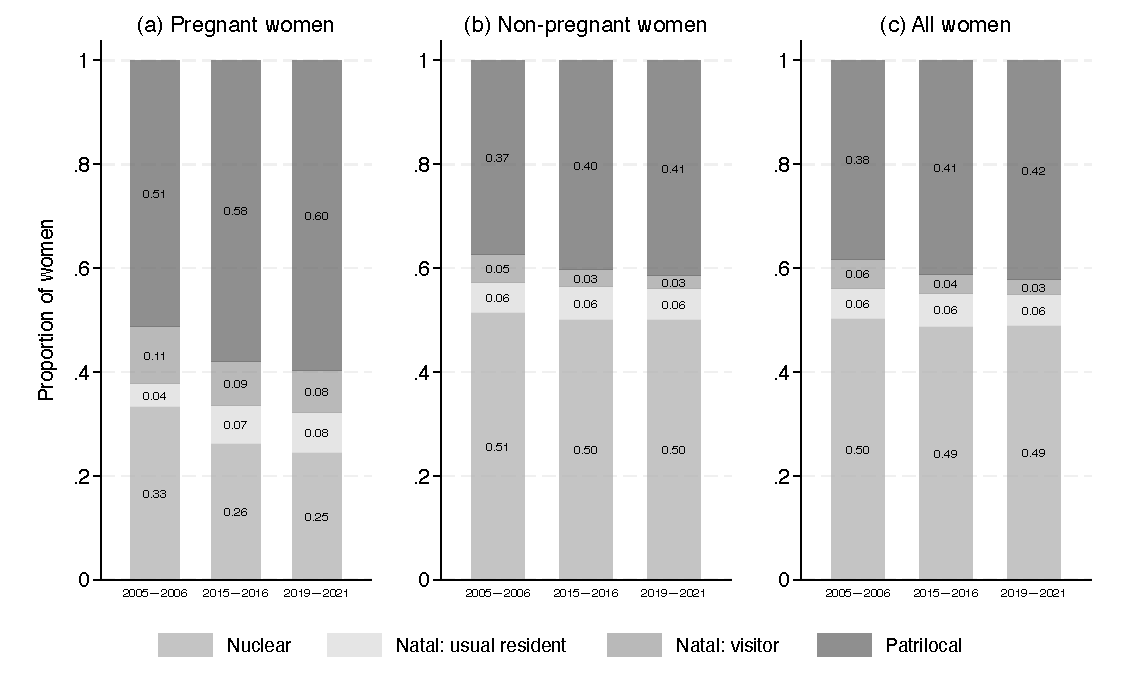
\includegraphics[scale=0.55]{figures/apdx bar graph three panel.pdf}
\end{center}

\vspace{1ex}
\small\scriptsize{\textsf{\textit{Note}: Data is from the NFHS rounds 3, 4, and 5. Panel A uses the sample of ever-married women who report being 3 or more months pregnant at the time of the survey. Panel B uses the sample of ever-married women who do not report being pregnant at the time of the survey. Panel C has no sample restrictions.}}

\end{flushleft}
\end{figure}


\begin{figure}[H]
\begin{flushleft}
\captionsetup{style=CAPFIG}
\caption{Household structure among married men whose wives are pregnant and not living with them}
\label{fig:hh_structure_men}
\vspace{0em}

\begin{center}
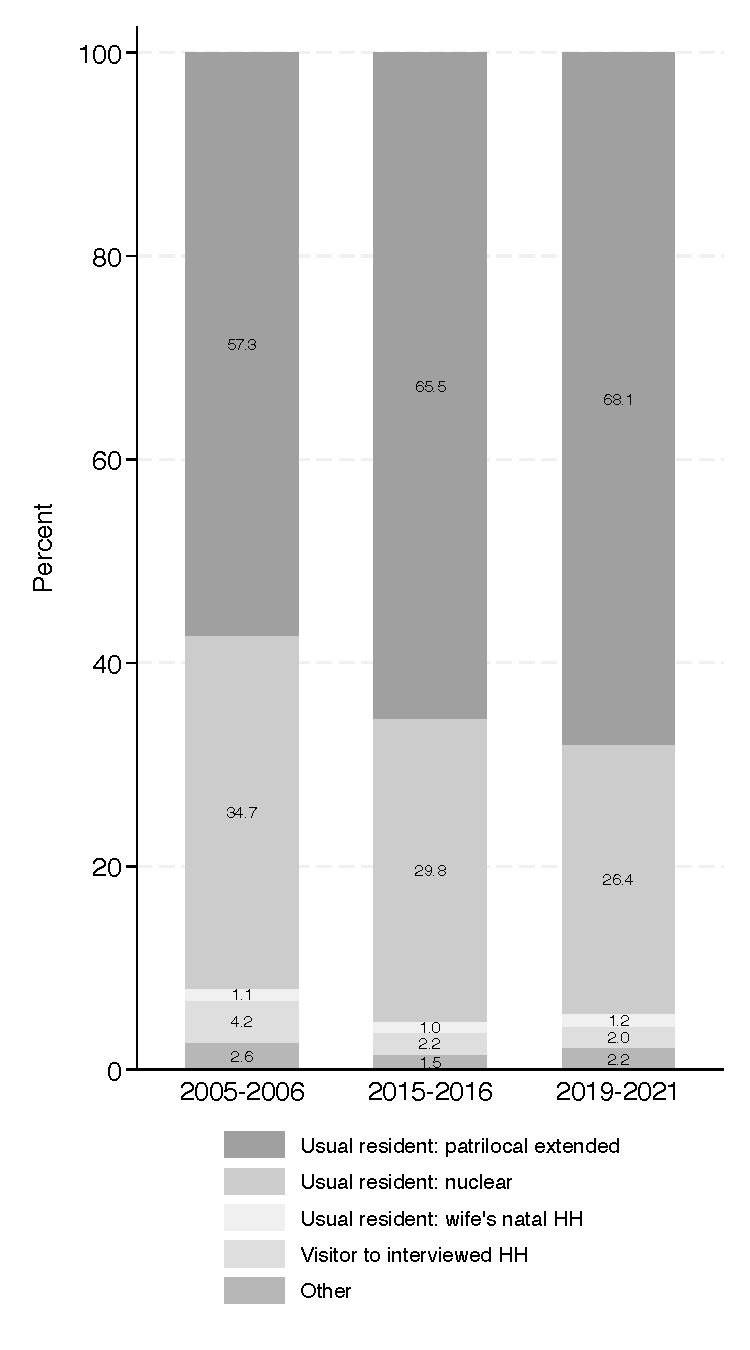
\includegraphics[width=0.95\textwidth]{figures/apdx bar graph three panel men.pdf}
\end{center}

\vspace{1ex}
\small\scriptsize{\textsf{\textit{Note}: Data is from NFHS rounds 3, 4, and 5. The sample is restricted to currently married men whose wife or partner was pregnant at the time of the survey and was staying elsewhere. Panel a shows the distribution of household structure among these men. Panel b shows the corresponding distribution among nonpregnant comparison cases, and panel c shows the distribution among all relevant married men, if included in the figure. Household structure categories are nuclear, patrilocal extended, and natal.}}

\end{flushleft}
\end{figure}

% ---------------------------------------------------------
% Appendix D
% ---------------------------------------------------------
\clearpage
\renewcommand{\thesection}{D-\arabic{section}}
\setcounter{equation}{0}
\renewcommand{\theequation}{D-\arabic{equation}}
\setcounter{figure}{0}
\renewcommand{\thefigure}{D-\arabic{figure}}
\setcounter{table}{0}
\renewcommand{\thetable}{D-\arabic{table}}

\subsection*{D. Kitagawa decomposition of changes in autonomy and health care indicators}

To assess whether changes in autonomy and maternal healthcare are driven by shifts in the distribution of household structure or by changes within household types, we implement a Kitagawa decomposition \citep{kitagawa1955components} comparing NFHS-3 (2005--06) and NFHS-5 (2019--21), using NFHS-3 as the baseline.

For each outcome $Y$, the change between NFHS-3 and NFHS-5 can be written as:

\begin{equation}
\Delta \equiv \bar Y^{5} - \bar Y^{3}
= \Delta_{\text{explained}} + \Delta_{\text{unexplained}}
\end{equation}

\begin{equation}
\Delta_{\text{explained}} =
\sum_{j \in \{N,P\}} \big(p_j^{5} - p_j^{3}\big)\frac{Y_j^{5} + Y_j^{3}}{2}
\end{equation}

\begin{equation}
\Delta_{\text{unexplained}} =
\sum_{j \in \{N,P\}} \big(Y_j^{5} - Y_j^{3}\big)\frac{p_j^{5} + p_j^{3}}{2}
\end{equation}

\begin{itemize}
    \item $j \in \{N,P\}$ indexes household type: nuclear ($N$) and patrilocal ($P$)
    \item $\bar Y^{3}$ and $\bar Y^{5}$ are the mean outcomes in NFHS-3 and NFHS-5
    \item $Y_j^{3}$ and $Y_j^{5}$ are the mean outcomes within household type $j$ in NFHS-3 and NFHS-5
    \item $p_j^{3}$ and $p_j^{5}$ are the proportions of women residing in household type $j$ in NFHS-3 and NFHS-5
\end{itemize}

\begin{table}[H]
\sansmath
\sffamily
\captionsetup{style=CAPTAB}
\caption{:  None of the improvement in the outcomes is explained by changing composition in household structures}
\label{tab:decomposition}
\vspace{-4pt}

\begin{scriptsize}
\setlength{\tabcolsep}{10pt}
\renewcommand{\arraystretch}{2.5}
\centering
\begin{tabular}{lccc}
\toprule
Outcome & \makecell{Total change\\(pp)} & \makecell{Share explained by \\household structure (\%)} & \makecell{Share from within-\\household structure changes (\%)} \\
\midrule
No say in own healthcare$^1$&-23.35&-1.72&101.72\\
No say in visits to family/friends$^1$&-28.27&-1.75&101.75\\
Four or more prenatal visits$^2$&22.24&1.15&98.85\\
Birth in a health facility$^2$&50.26&0.54&99.46\\
\bottomrule
\end{tabular}

\end{scriptsize}

\vspace{1ex}
\small\scriptsize{\textsf{\textit{Note}: Data is from the NFHS rounds 3, 4, and 5.}}
\newline\small\scriptsize{\textsf{$^1$ The sample is restricted to ever-married women who report being three or more months pregnant at the time of the survey, and those who are living in either nuclear or patrilocal extended households.}}
\newline\small\scriptsize{\textsf{$^1$ The sample is restricted to ever-married women who report having given birth in the last 3 to 12 months, and those who are living in either nuclear or patrilocal extended households.}}

\end{table}

%%%%%%%%%%%%%%%%%%%%%% END APPENDIX %%%%%%%%%%%%%%%%%%%%%%%%%%

% Ensure that there is an even number of pages. 
\cleardoublepage
\end{document}


